
%%%%%%%%%%%%%%%%%%%%%%%%%%%%%%%%%%%%%%%%%%%%%%%%%%
% Basic setup. Most papers should leave these options alone.
\documentclass[fleqn,usenatbib]{mnras}

\usepackage[T1]{fontenc}
\DeclareRobustCommand{\VAN}[3]{#2}
\let\VANthebibliography\thebibliography
\def\thebibliography{\DeclareRobustCommand{\VAN}[3]{##3}\VANthebibliography}

%%%%% AUTHORS - PLACE YOUR OWN PACKAGES HERE %%%%%
\usepackage{graphicx}	% Including figure files
\usepackage{amsmath}	% Advanced maths commands
\usepackage{amssymb}	% Extra maths symbols
\usepackage{xspace} 
\usepackage{xcolor}
\usepackage{upgreek}
\usepackage{CJK}
\usepackage{fontawesome}
\usepackage{gensymb}
\usepackage{multirow}
\usepackage{mathtools}
\usepackage{newtxtext,newtxmath}

%%%%% AUTHORS - PLACE YOUR OWN COMMANDS HERE %%%%%
\newcommand{\ToDo}[1]{\textbf{\textcolor{blue}{ToDo: #1}}}
\newcommand{\SB}[1]{{\textcolor{orange}{SB: #1}}}
\newcommand{\LM}[1]{{\textcolor{purple}{LM: #1}}}
\newcommand{\TB}[1]{{\textcolor{green}{TB: #1}}}
\newcommand{\Gaia}{\textit{Gaia}\xspace} % \Gaia

%%%%%%%%%%%%%%%%%%%%%%%%%%%%%%%%%%%%%%%%%%%%%%%%%%
%%%%%%%%%%%%%%%%%%% TITLE PAGE %%%%%%%%%%%%%%%%%%%

% Title of the paper, and the short title which is used in the headers.
% Keep the title short and informative.
\title[NIHAO vs. Milky Way: Radial metallicity gradients]{More than just a line: Shining light on the radial metallicity gradient with NIHAO simulations}

% The list of authors, and the short list which is used in the headers.
% If you need two or more lines of authors, add an extra line using \newauthor
\author[S. Buder]{
S. Buder,$^{1,2}$\thanks{E-mail: sven.buder@anu.edu.au}
\\
% List of institutions
$^{1}$Research School of Astronomy \& Astrophysics, Australian National University, ACT 2611, Australia\\
$^{2}$Center of Excellence for Astrophysics in Three Dimensions (ASTRO-3D), Australia\\
}

% These dates will be filled out by the publisher
\date{Accepted YYYY Month DD. Received YYYY Month DD}

% Enter the current year, for the copyright statements etc.
\pubyear{2024}

% Don't change these lines
\begin{document}
\label{firstpage}
\pagerange{\pageref{firstpage}--\pageref{lastpage}}
\maketitle

% Abstract of the paper
\begin{abstract} % XXX words
ABSTRACT HERE
\end{abstract}
% Select between one and six entries from the list of approved keywords.
% Don't make up new ones.
\begin{keywords}
cosmology: observations -- Galaxy: formation -- Galaxy: evolution -- Galaxy: abundances
\end{keywords}

%%%%%%%%%%%%%%%%%%%%%%%%%%%%%%%%%%%%%%%%%%%%%%%%%%

%%%%%%%%%%%%%%%%% BODY OF PAPER %%%%%%%%%%%%%%%%%%

\section{Introduction}
\label{sec:intro}

\textbf{Great insight thanks to \textit{Gaia} into the radial metallicity gradient}. Specifically point out:
\begin{itemize}
    \item \citet{Eilers2019}
    \item \citet{Poggio2021}
    \item \citet{Poggio2022} especially Fig. 2!
    \item \citet{Imig2023}
    \item \citet{Chen2023} - see their Figs. 4-6 with lots of (expected?) scatter
    \item \citet{Hackshaw2024}
\end{itemize}

\textbf{FINE STRUCTURE OF THE METALLICITY GRADIENT} \citep{Genovali2014}

"Over the past decade, different authors using different observational tools often came to contradictory views on both the shape, the magnitude and the evolution of the abundance gradients along the disk" \citep{Chiappini2002}.

\begin{itemize}
    \item \textbf{Galactic Chemical Evolution}
    \begin{itemize}
        \item It matters if/how linear the radial abundance gradient is to test galactic chemical evolution models \citep[see e.g.][]{Chiappini2001}, especially in the outer regions of our Galaxy \citep{Chiappini2002}.
        \item \citet{Minchev2014b}
        \item \citet{Kubryk2015}
        \item \citet{Stanghellini2015}
        \item \citet{Matteucci2001b}
    \end{itemize}
    \item \textbf{Observations in the Milky Way}
    \begin{itemize}
        \item see references in Table 1 by \citet{Chiappini2001}
        \item with RAVE and Geneva-Copenhagen Survey \citep{Boeche2013}
        \item with APOGEE \citep{Anders2014, Cunha2016} 
        \item with \textit{Gaia-ESO} \citep{Bergemann2014}. \citet{Bergemann2014} find $\Delta \mathrm{[Fe/H]} / \Delta R = -0.068 \pm 0.014 \mathrm{dex kpc^{-1}}$ close to the plane ($\vert Z \vert < 300\,\mathrm{pc}$).
        \item \citet{Willett2023}
    \end{itemize}
    \item \textbf{Observations outside the Milky Way}
    \begin{itemize}
        \item \citet[][see their Figs. 5 and 11]{Sanchez2014} with CALIFA galaxies 12 + log(O/H) vs. R/Re
        \item \citet{Mun2024} not explicitely radius vs. [Fe/H], but MAGPI
        \item \citet{Chen2024} (see their Fig. 6) on the effects of spiral arms on different tracers of the interstellar medium and stellar populations
        \item \citet{Chen2023} see their Figs. 4-6.
    \end{itemize}
    \item Problems with Observations:
    \begin{itemize}
        \item "One of the most difficult but fundamental tasks is to assess the completeness of the observed dataset." \citep{Bergemann2014}
        \item different samples find different gradients. Compare e.g. steeper gradients by \citet{Bergemann2014, Boeche2013} with \citet{AllendePrieto2006, Hayden2014, Anders2014, Katz2011}.
        \item "but this could reflect our small dataset or the fact that the studies probe much larger $\vert Z \vert$." \citep{Bergemann2014}.
        \item Spiral arms \citet{Poggio2021}: Galactic spiral structure revealed by Gaia EDR3
        \item Spiral arms \citet{Poggio2022}: The chemical signature of the Galactic spiral arms revealed by Gaia DR3
        \item Galactic warp \citep[e.g.][]{Lemasle2022}
    \end{itemize}
    \item Which tracers do you use?
    \begin{itemize}
        \item Open clusters?
        \item Cepheids? \citep{Andrievsky2002, Andrievsky2002b, Lemasle2007, Lemasle2013}
        \item OB stars?
        \item H II regions?
    \end{itemize}
    \item Simulations
    \begin{itemize}
        \item \citet{Minchev2014b}
        \item \citep[Figs. 7 and 9 from][]{Agertz2021}
        \item \citep[Figs. 6 and 9 from][]{Ma2017} % The structure and dynamical evolution of the stellar disc of a simulated Milky Way-mass galaxy
        \item \citep[Fig. 1 from][]{Pilkington2012} % Metallicity gradients in disks. Do galaxies form inside-out?
        \item Fig. 4 from \citet{Tissera2019} % The oxygen abundance gradients in the gas discs of galaxies in the EAGLE simulation
        \item \cite{Brook2012} % Thin disc, thick disc and halo in a simulated galaxy
        \item Bellardini
        \begin{itemize}
            \item \cite{Bellardini2021}
            \item \citet{Bellardini2022}
            \item \cite{Carrillo2023} did not exactly look into this, but had Fig. 13 showing radial metallicity gradient (for 5 Gyr old stars)
            \item \citep{Graf2024}  
        \end{itemize}
        \item Metha
        \begin{itemize}
            \item \cite{Metha2021}
            \item \cite{Metha2022}
            \item \cite{Metha2023}
            \item \cite{Metha2024}
            \item \cite{Metha2024b}
        \end{itemize}
    \end{itemize}
\end{itemize}


...

The paper is structured as follows: Sec.~\ref{sec:data} describes the data of GALAH observations and NIHAO simulations. Sec.~\ref{sec:radial_metallicity_gradients} analyses the radial metallicity gradients of the simulations. Sec.~\ref{sec:discussion} discusses to which extend these gradients are linear and what we can learn from the residuals. Sec.~\ref{sec:conc} concludes the paper.

\section{Data: Observations and simulations} \label{sec:data}

\subsection{Observational data from the GALAH Survey}\label{sec:obs_data}

% Observations are provided through the GALactic Archaeology with HERMES (GALAH) survey. For our study, we use the abundance measurements from the third data release (DR3) of the GALAH Survey with its 588,571 stars \citep{Buder2021}. The main program of the survey targets nearby stars via their visual magnitudes (typically $9 < V < 12$ and $12 < V < 14$) while neglecting the Galactic plane ($\vert b \vert > 10\,\mathrm{deg}$). However, the data release also includes auxiliary programs of the K2 and TESS footprints \citep{Sharma2018, Sharma2019} as well as open and globular clusters \cite[for more details see][]{Buder2021}. Stars were targeted with the 2dF fibre optics positioner system at the Anglo-Australian Telescope \citep{Heijmans2012, Farrell2014} and the light of up to 400 stars was simultaneously fed into the High Efficiency and Resolution Multi-Element Spectrograph \citep[HERMES,][]{Barden2010, Sheinis2015}. HERMES delivers high-resolution ($R \sim 28,000$) spectra in four wavelength bands across the optical range which were reduced with the pipeline by \citep{Kos2017}.

% Stellar parameters ($T_\text{eff}$, $\log g$, [Fe/H], $v_\text{mic}$, $v_\text{broad}$, and $v_\text{rad}$) and abundances for up to 31\footnote{Li*, C*, O*, Na*, Mg*, Al*, Si*, K*, Ca*, Sc, Ti, V, Cr, Mn*, Fe*, Co, Ni, Cu, Zn, Rb, Sr, Y, Zr, Mo, Ru, Ba*, La, Ce, Nd, Sm, and Eu, with * denoting elements calculated in 1D non-local thermodynamic equilibrium (non-LTE), instead of 1D LTE.} different elements across multiple nucleosynthesis channels are estimated using a modified version of the spectrum synthesis code Spectroscopy Made Easy \citep[\textsc{sme}][]{Valenti1996, Piskunov2017} and 1D \textsc{marcs} model atmospheres \citep{Gustafsson2008}. Eleven elements are computed in non-LTE \citep{Amarsi2020}, the others in local thermodynamic equilibrium (LTE), and additional constraints on the surface gravities are incorporated through inferred distances by \citet{BailerJones2021} and their limit on absolute magnitudes and luminosities.

% In addition to the chemical information, we use the crossmatches of stars with value-added-catalog for stellar ages. The latter incorporates photometric and astrometric information from \Gaia eDR3 \citep{Lindegren2021a} and 2MASS \citep{Skrutskie2006} to estimate isochrone ages with the \textsc{bstep} code \citep{Sharma2018}.

% We apply the following general quality and selection cuts to the data, firstly $\texttt{flag\_repeat} = 0$ to get one measurement per star, and secondly $\texttt{flag\_sp} = 0$, $\texttt{flag\_fe\_h} = 0$, $\texttt{flag\_Mg\_fe} = 0$, $\texttt{snr\_c2\_iraf} > 25$, and $\mathrm{[Fe/H]} > -2$ to get the most reliable stellar parameters while maintaining a sufficient amount of stars. Whenever we use additional elemental abundances of an element X, we also enforce $\texttt{flag\_X\_fe} = 0$.

% While we have considered enforcing \textsc{bstep} age uncertainties below 50\%, we have decided against implementing a sharp limit, both to avoid complex influences\footnote{Of the \input{tex_text/age_above_8gyr.tex} stars above $8\,\mathrm{Gyr}$ \input{tex_text/age_above_8gyr_above50perc_ageunc}, \input{tex_text/age_above_8gyr_above40perc_ageunc}, and \input{tex_text/age_above_8gyr_above30perc_ageunc} have uncertainties above $50\%$, $40\%$, and $30\%$, respectively. Of the \input{tex_text/age_below_8gyr.tex} stars below $8\,\mathrm{Gyr}$ already \input{tex_text/age_below_8gyr_above50perc_ageunc.tex} have uncertainties above $50\%$.} in the selection function and because it does not significantly impact the stars with ages above $8\,\mathrm{Gyr}$.

% To allow better comparability with the simulations later on (see Sec.~\ref{sec:location}), we also limit our sample to stars with Galactic latitude $\vert b \vert > 10\,\mathrm{deg}$ and distance $D_\varpi < 4.2\,\mathrm{kpc}$ \citep[based on photogeometric distances from][]{BailerJones2021}, the 95th distance percentile of GALAH DR3 \citep{Buder2021}. After applying all these cuts, our sample still consists of \input{tex_text/nr_stars_in_galah_after_cuts}stars, allowing a statistically meaningful comparison with theoretical predictions.

\subsection{Theoretical predictions from a NIHAO Zoom-in simulation}\label{sec:sim_data}

The model perspective on accretion is provided through a cosmological zoom-in simulation of a Milky Way analogue (\texttt{g8.26e11}) from the \textit{Numerical Investigation of a Hundred Astronomical Objects} \citep[NIHAO,][]{Wang2015}. The model galaxy has a total mass (gas, stars and dark matter) of $8.26 \cdot 10^{11}\,\mathrm{M_\odot}$ and contains $4 \cdot 10^{10}\,\mathrm{M_\odot}$ stellar mass with a stellar mass resolution of $1.06 \cdot 10^{5}\,\mathrm{M_\odot}$ \citep{Buck2021} and was calculated as part of the NIHAO-UHD project \citep{Buck2020b}.

\subsubsection{How simulations were carried out}

% Simulations were carried out with the smoothed particle hydrodynamics code \texttt{Gasoline2} \citep{Wadsley2017} using cosmological parameters from \citet{Planck2014} with initial conditions and energetic feedback descriptions from the NIHAO project \citep{Wang2015}. Zoom-in simulations were then performed as described in detail by \citet{Buck2021} with star formation following \citet{Stinson2006} and energetic feedback following \citet{Stinson2013}.

% Because computational resources still limit the mass resolution of simulations, we are relying on tracer particles that represent simple stellar populations (SSPs) with the same age, overall metallicity and discrete initial mass function (IMF). \citet{Buck2021} have implemented the flexible chemical evolution code \textsc{chempy} \citep{Rybizki2017} to calculate the chemical yields for the SSPs. In particular, we use the alternative (\texttt{alt}) setup of \textsc{chempy} that assumes a \citet{Chabrier2003} IMF with high-mass slope of $\alpha_\text{IMF} = -2.3$ over a mass range of $0.1-100\,\mathrm{M_\odot}$ for SSPs across a metallicity range of $Z/Z_\odot \in [10^{-5},2]$. The code calculates the contribution from asymptotic giant branch (AGB) stars, CCSN across a mass range of $8-40\,\mathrm{M_\odot}$, and SNIa with a an exponential function with exponent $-1.12$, a delay time of $40\,\mathrm{Myr}$, and a normalization of the SNI rate of -2.9. For each of these nucleosynthetic channels, yields from the following studies are used: \citet{Limongi2018} for CCSN, \citet{Seitenzahl2013} for SNIa, and \citet{Karakas2016} for AGB stars.

% To achieve a roughly similar selection as the observational data (see Secs.~\ref{sec:obs_data} and \ref{sec:location}), while maintaining enough star particles, we limit the simulated data set to star particles within a torus at $8.2\,\mathrm{kpc}$ galactocentric radius with a $4.2\,\mathrm{kpc}$ tube radius (corresponding to the 95th distance percentile of the GALAH sample) and neglect star particles within $\vert b \vert~<~10\,\mathrm{deg}$ or $\mathrm{[Fe/H]} < -2$. We use the last simulation snapshot at a cosmic time of $13.8\,\mathrm{Gyr}$ to estimate the ages from the reported formation time.

% The simulation traces the elemental abundances of H, He, C, N, O, Ne, Mg, Al, Si, P, S, V, Cr, Mn, Fe, Co, and Ba. Of these, ten correspond with the GALAH data and allow us to compare diagnostic plots possible with abundances of C, O, Mg, Al, Si, V, Cr, Mn, Co and Ba. To allow a better comparison of simulated to observed abundance patterns, we shift the abundance patterns [X/H] by the values listed in Table~\ref{tab:shift_4to5gyr}, such that the median abundance for [X/H] is Solar for the stars with ages of Solar age ($4-5\,\mathrm{Gyr}$) in the GALAH-like footprint of the Milky Way analogue.

% The simulation records galactocentric Cartesian positions $(X,Y,Z)$ and velocities $(V_X,V_Y,V_Z)$ for each particle, which we transform into a galactocentric Cylindrical coordinate frame via
% \begin{align}
%     R = \sqrt{X^2 + Y^2} \qquad &\& \qquad V_R = \frac{X*V_X + Y*V_Y}{R} \\
%     \phi = \arctan(X/Y) \qquad &\& \qquad V_\phi = \frac{-Y*V_X + X*V_Y}{R} \\
%     z = Z  \qquad &\& \qquad V_z = V_Z,
% \end{align}
% while using the \textsc{numpy} \textsc{arctan2} package.

% \begin{table}
%     \centering
%     \caption{
%     \textbf{Median abundance [X/H] for particles of the Milky Way analogue with $4 < \mathrm{Age~/~Gyr} < 5$ in the observation footprint.}
%     These were used to shift the the abundance to agree with an expected Solar value.
%     }
%     \input{tables/tabular_shift_by_4_to_5_gyr.tex}
%     \label{tab:shift_4to5gyr}
% \end{table}

\SB{Show the X-Y and R-z distribution -> This will be important when we select stars to make sure we select close to the galactic plane! Also compare with \citet{Poggio2022} on how they did it (if they applied a cut in $\vert z \vert$, maybe they only did an age cut?)!}

%%%%%%%%%%%%%%%%%%%%%%%%%%%%%%%%%%%%%%%%%%%%%%%%%%

\section{Radial metallicity gradients in NIHAO}
\label{sec:radial_metallicity_gradients}

\begin{figure*}
    \centering
    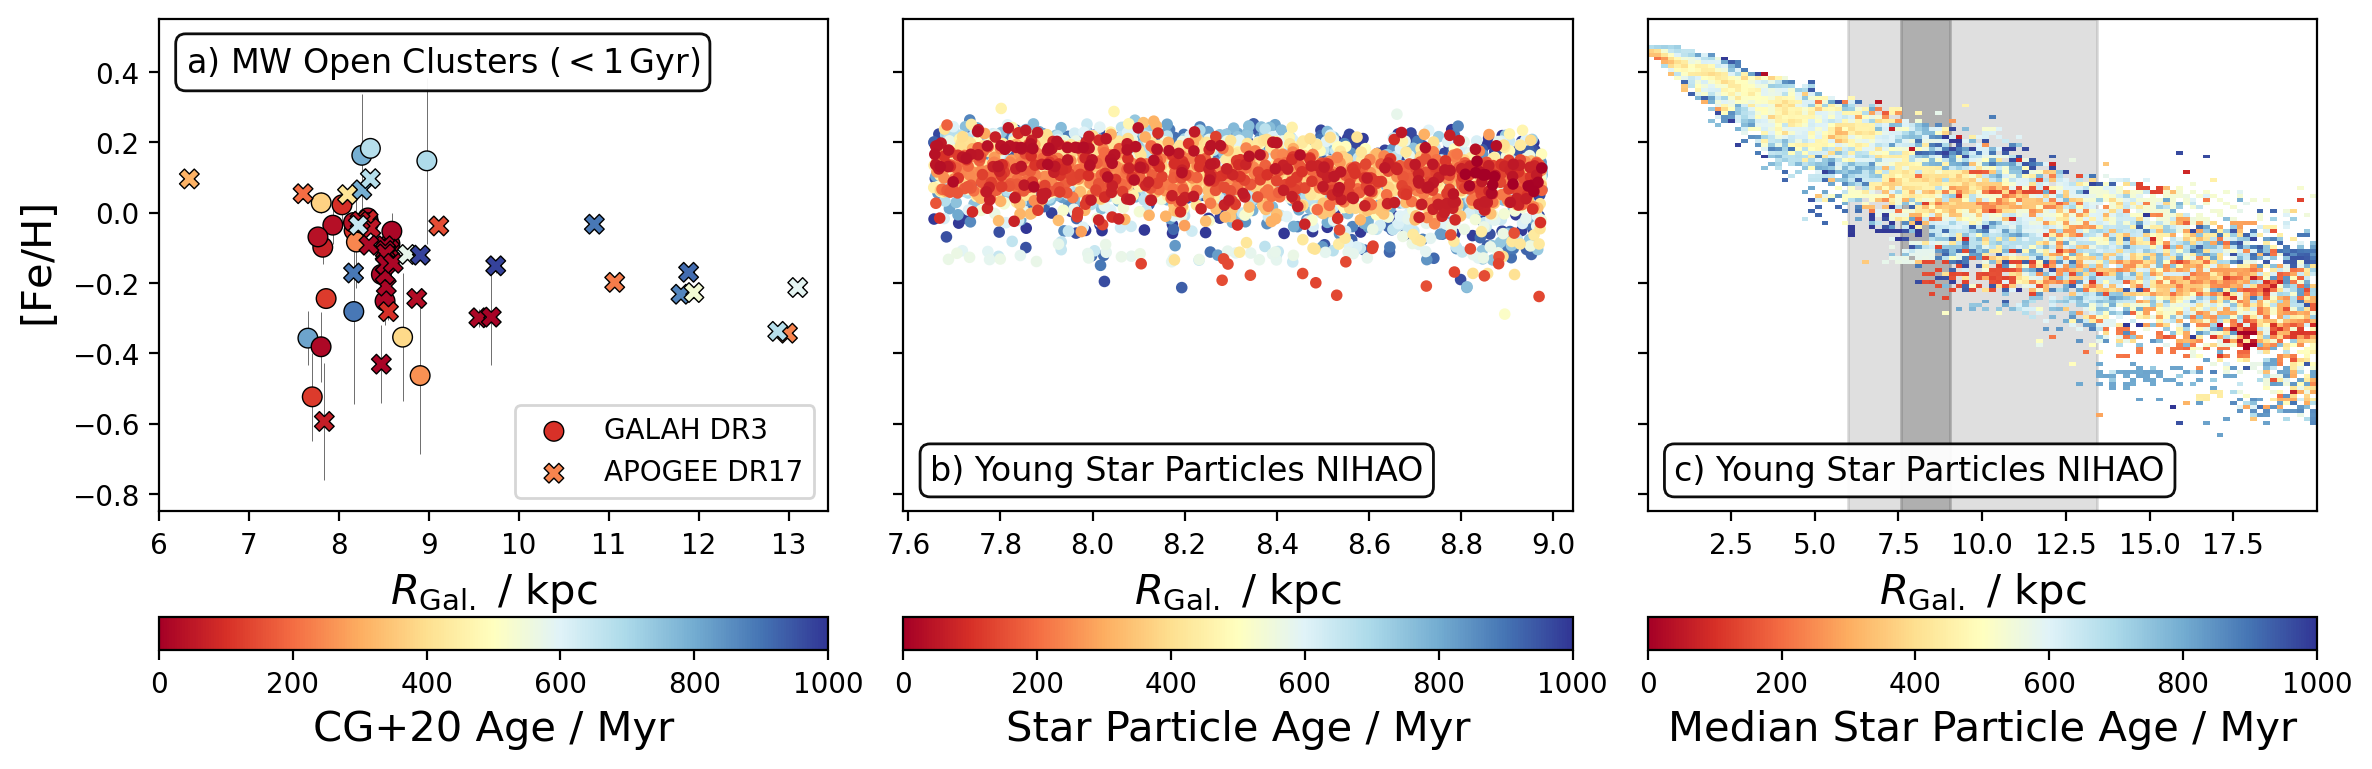
\includegraphics[width=\textwidth]{figures/radial_metallicity_gradients_mw_vs_nihao.png}
    \caption{Caption}
    \label{fig:radial_metallicity_gradients_mw_vs_nihao}
\end{figure*}


\subsection{Linear radial metallicity gradients}
\label{sec:linear_radial_metallicity_gradients}

\subsection{Deviations from the linear radial metallicity gradients}
\label{sec:deviations_radial_metallicity_gradients}

\begin{figure*}
    \centering
    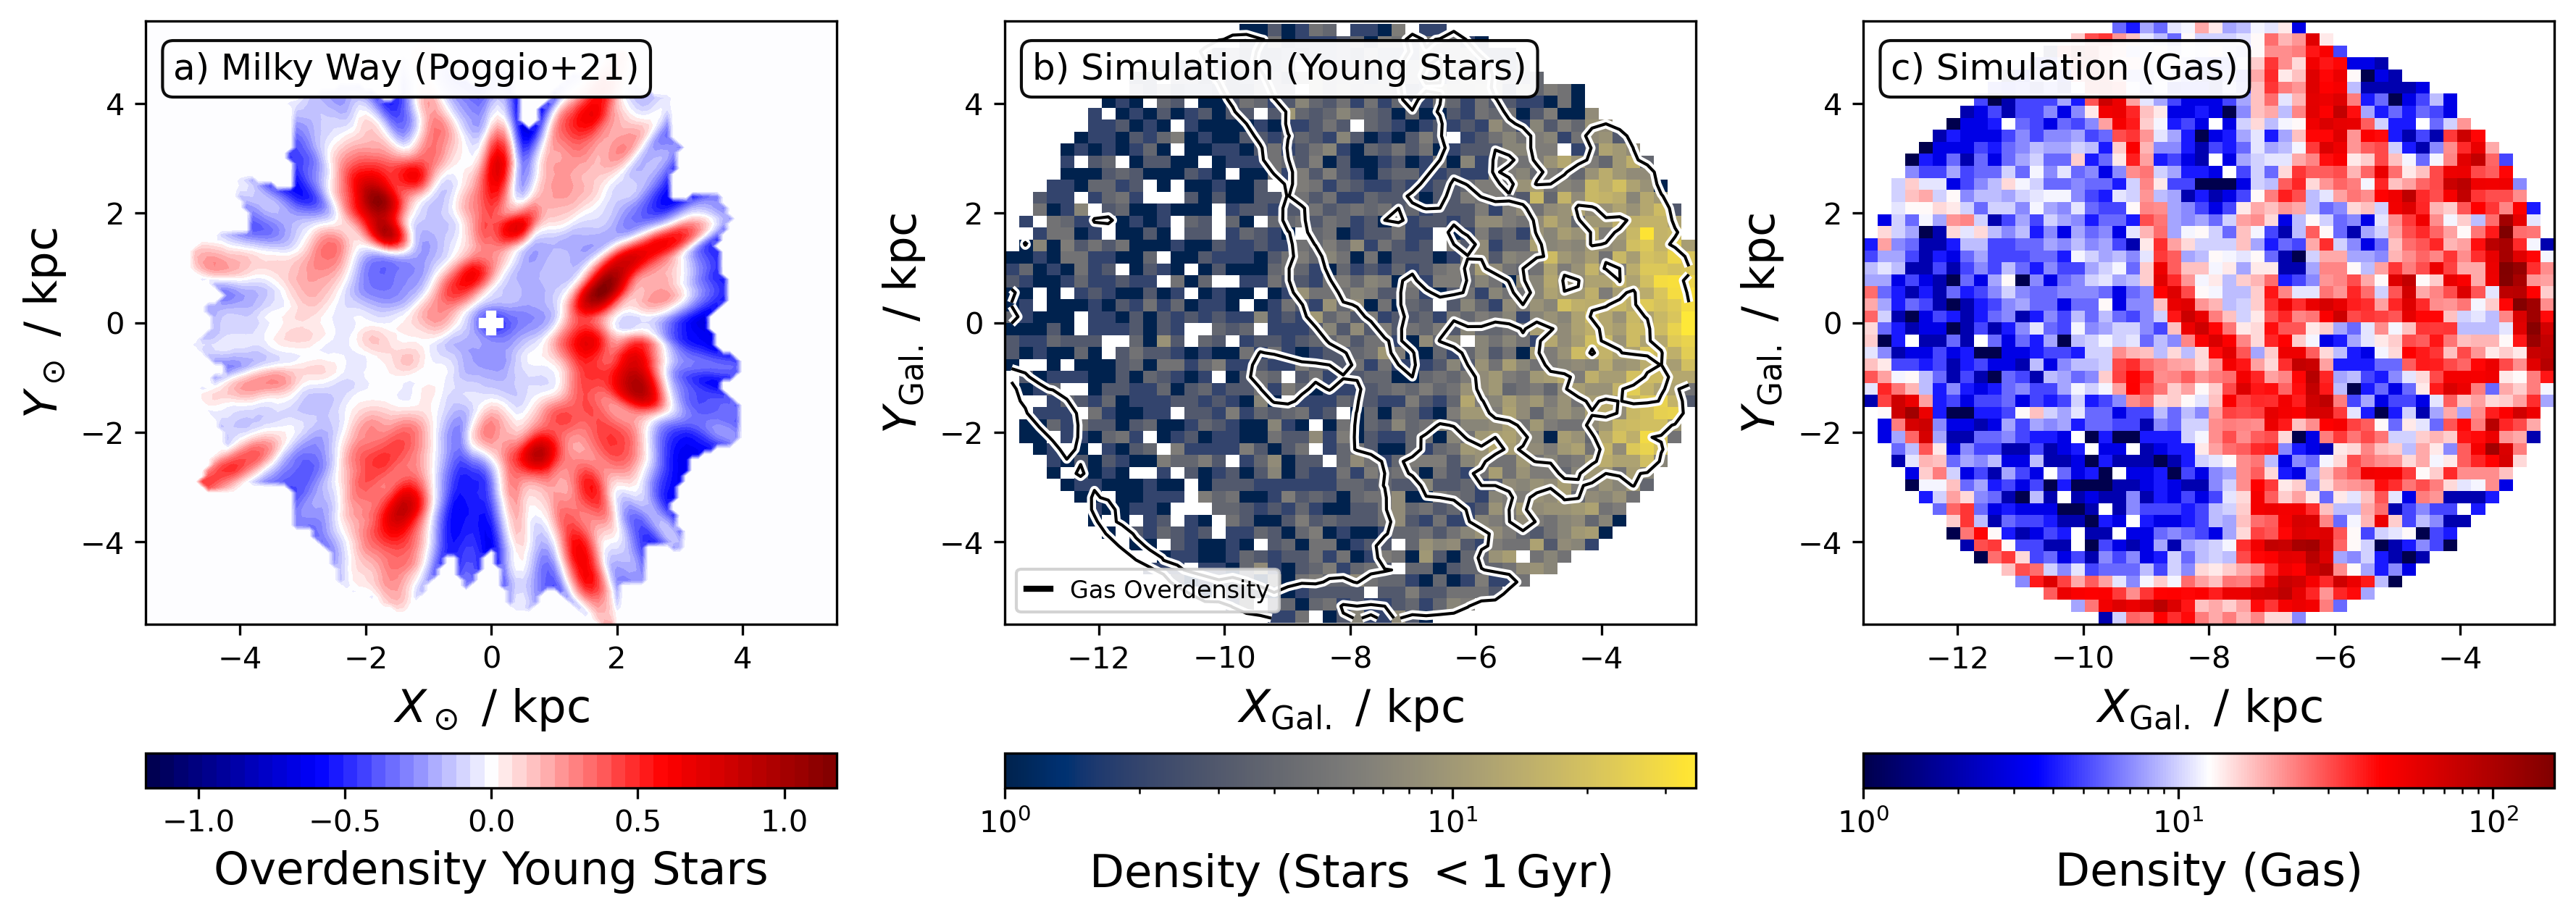
\includegraphics[width=\textwidth]{figures/overdensities_mw_vs_nihao.png}
    \caption{Caption}
    \label{fig:overdensities_mw_vs_nihao}
\end{figure*}

\section{Radial metallicity gradients in comparison}
\label{sec:radial_metallicity_gradient_comparison}

\begin{figure*}
    \centering
    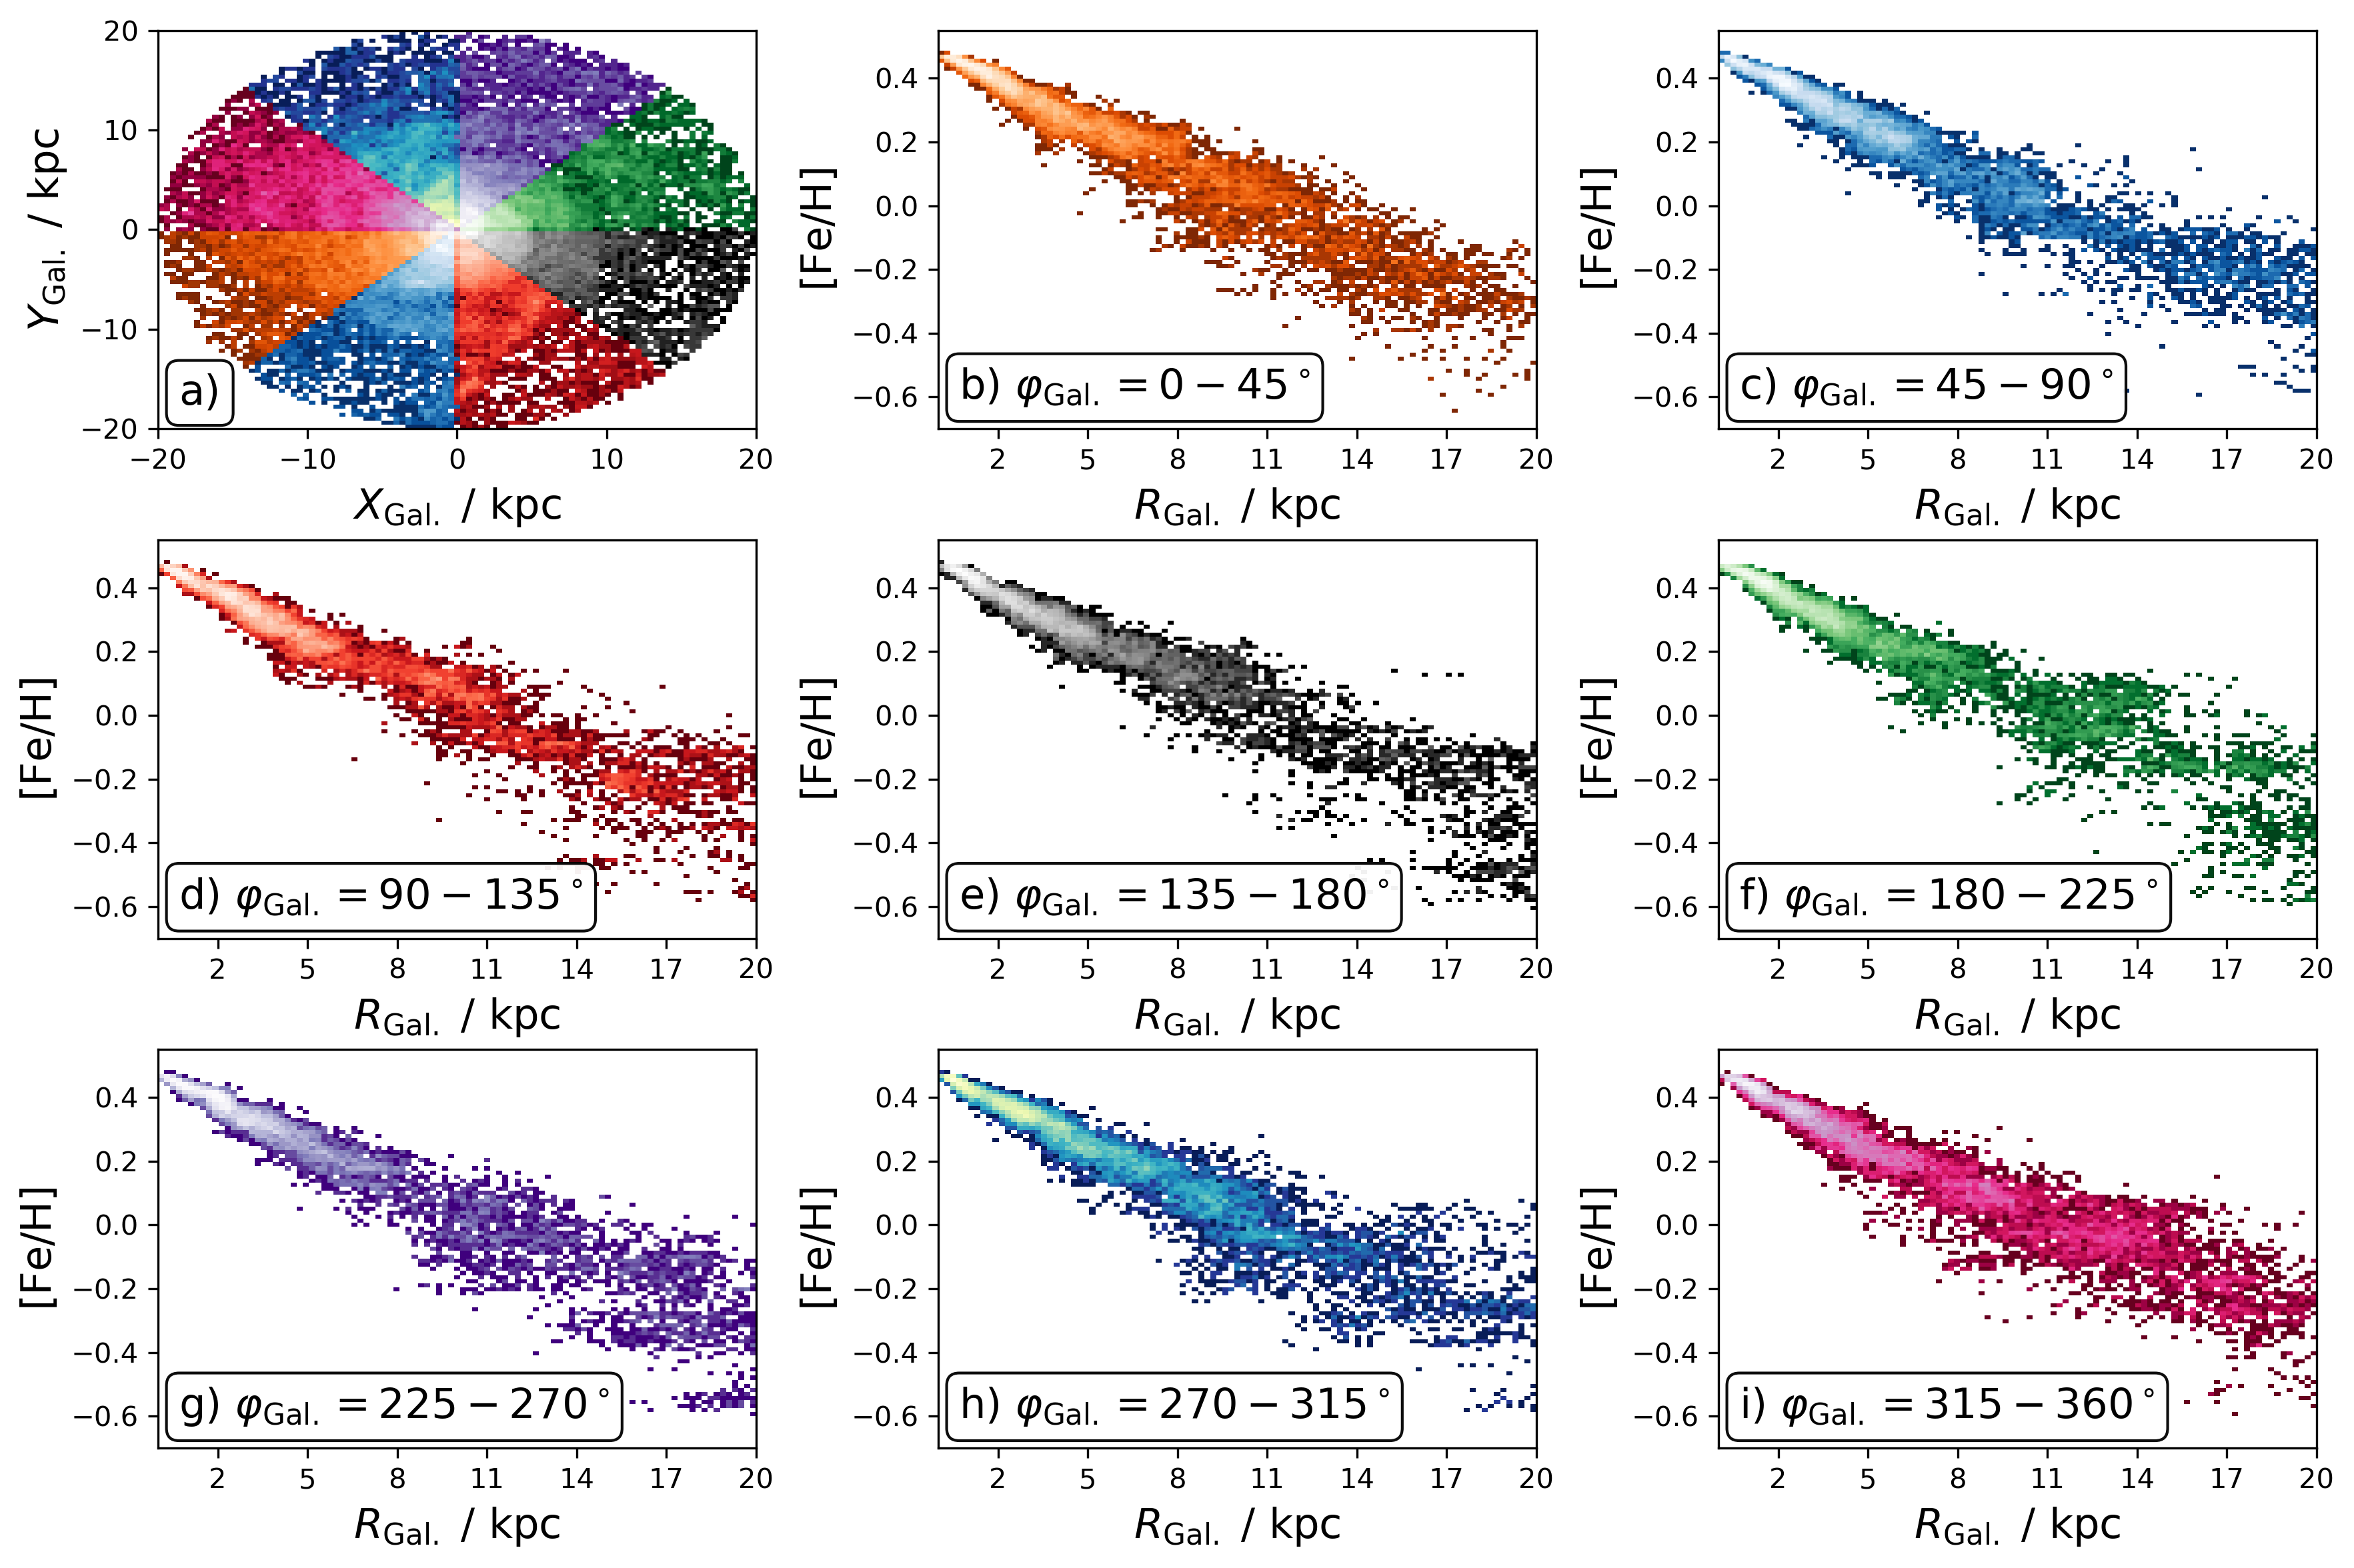
\includegraphics[width=\textwidth]{figures/radial_metallicity_gradients_mw_in_angles.png}
    \caption{Density variation of the radial metallicity gradient $R-\mathrm{[Fe/H]}$ across 8 different sectors. A rotating lighthouse-like GIF animation of the median age and median density of the $R-\mathrm{[Fe/H]}$-relation is freely available on the \href{https://github.com/svenbuder/nihao_radial_metallicity_gradients/blob/main/figures/xyz_rfeh.gif}{github repository}.}
    \label{fig:radial_metallicity_gradients_mw_in_angles}
\end{figure*}

\SB{Do the same as Fig.~\ref{fig:radial_metallicity_gradients_mw_in_angles}, but with bins colored by median age.}

\SB{Calculate global $R-\mathrm{[Fe/H]}$, then local for the 8 sectors of Fig.~\ref{fig:radial_metallicity_gradients_mw_in_angles}, plot both in 2x4 subpanels, and color-code the density plots by median deviation from this line with a seismic map.}


\begin{figure*}
    \centering
    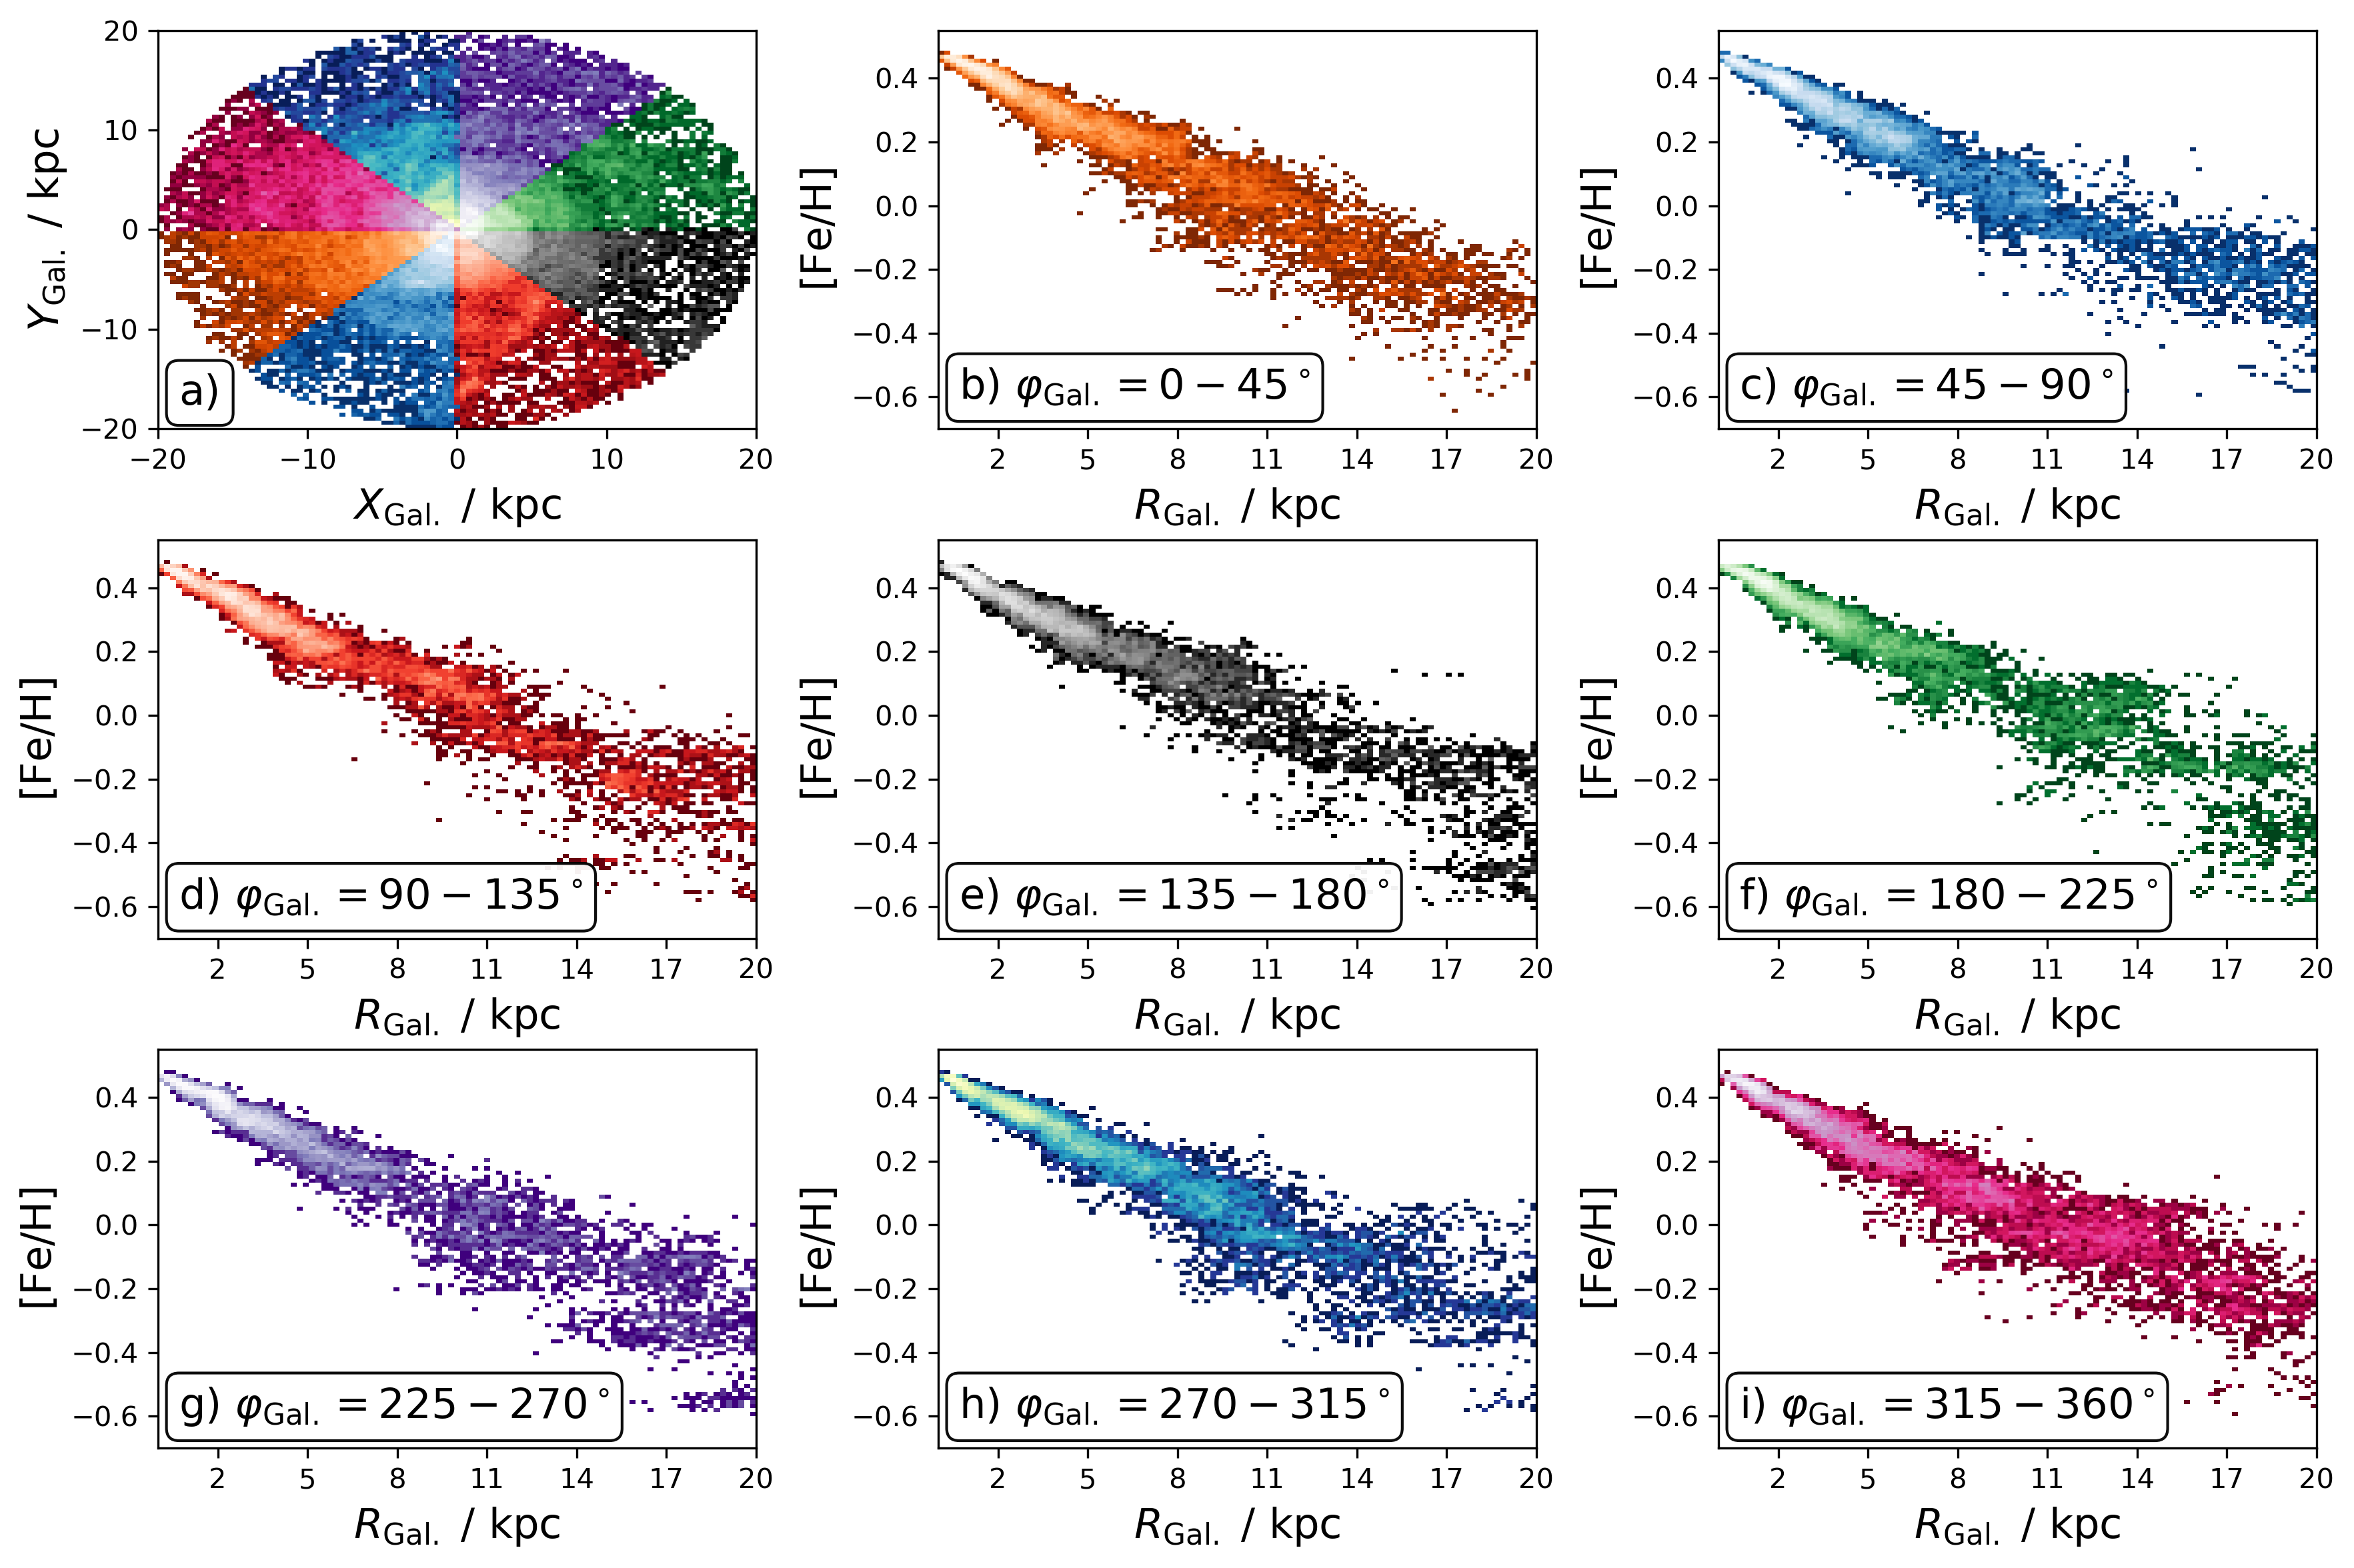
\includegraphics[width=\textwidth]{figures/radial_metallicity_gradients_mw_in_angles.png}
    \caption{Density variation of the radial metallicity gradient $R-\mathrm{[Fe/H]}$ across full stellar disk and 8 different sectors (same panel order as for Fig.~\ref{fig:radial_metallicity_gradients_mw_in_angles}). Linear radial metallicity gradients have been fit globally (red dashed line) and for each sector with colors following the same color code as in Fig.~\ref{fig:radial_metallicity_gradients_mw_in_angles}}.
    \label{fig:linear_radial_metallicity_gradients_mw_in_angles}
\end{figure*}

Fig.~\ref{fig:linear_radial_metallicity_gradients_mw_in_angles}f shows impressively, that if you look at a rather narrow range of $R_\mathrm{gal}$, such as $5 < R_\mathrm{gal} < 15\,\mathrm{kpc}$, the radial metallicity gradient could actually look like it is damping towards larger radii. \SB{Is this possibly what is happening in local studies of our galaxy, where many researchers are actually fitting 2 linear gradients with a break radius?}

%%%%%%%%%%%%%%%%%%%%%%%%%%%%%%%%%%%%%%%%%%%%%%%%%%
\section{Discussion} \label{sec:discussion}

Comparison to \citet[][see their Fig. 10]{Minchev2014b}: They see significant decrease of stars towards larger radii (note to myself: their bins are not scatter, but number density in Fig. 10). How does this compare to our number densities?


%%%%%%%%%%%%%%%%%%%%%%%%%%%%%%%%%%%%%%%%%%%%%%%%%%
%%%%%%%%%%%%%%%%%%%%%%%%%%%%%%%%%%%%%%%%%%%%%%%%%%
\section{Conclusions}
\label{sec:conc}


\section*{Acknowledgements}

We acknowledge the traditional owners of the land on which the AAT and ANU stand, the Gamilaraay, the Ngunnawal and Ngambri people. We pay our respects to elders past, present, and emerging and are proud to continue their tradition of surveying the night sky in the Southern hemisphere.

This work was supported by the Australian Research Council Centre of Excellence for All Sky Astrophysics in 3 Dimensions (ASTRO 3D), through project number CE170100013. SB acknowledges support from the Australian Research Council under grant number DE240100150 which enabled SB to continue researching at the end of a fixed-term position and finalising this study. TB acknowledges funding from the Carl Zeiss Stiftung and support from the European Research Council under ERC-CoG grant CRAGSMAN-646955. We gratefully acknowledge the Gauss Centre for Supercomputing e.V. (\url{www.gaus s-centre.eu}) for funding this project by providing computing time on the GCS Supercomputer SuperMUC at Leibniz Supercomputing Centre (\url{www.lrz.de}). Simulations were partially computed with High Performance Computing resources at New York University, Abu Dhabi.

\section*{Facilities}

\textbf{AAT with 2df-HERMES at Siding Spring Observatory:} The GALAH Survey is based data acquired through the Australian Astronomical Observatory, under programs: A/2013B/13 (The GALAH pilot survey); A/2014A/25, A/2015A/19, A2017A/18 (The GALAH survey phase 1), A2018 A/18 (Open clusters with HERMES), A2019A/1 (Hierarchical star formation in Ori OB1), A2019A/15 (The GALAH survey phase 2), A/2015B/19, A/2016A/22, A/2016B/10, A/2017B/16, A/2018B/15 (The HERMES-TESS program), and A/2015A/3, A/2015B/1, A/2015B/19, A/2016A/22, A/2016B/12, A/2017A/14, (The HERMES K2-follow-up program). This paper includes data that has been provided by AAO Data Central (\url{datacentral.aao.gov.au}).

\textbf{\Gaia: } This work has made use of data from the European Space Agency (ESA) mission \Gaia (\url{http://www.cosmos.esa.int/gaia}), processed by the \Gaia Data Processing and Analysis Consortium (DPAC, \url{http://www.cosmos.esa.int/web/gaia/dpac/consortium}). Funding for the DPAC has been provided by national institutions, in particular the institutions participating in the \Gaia Multilateral Agreement. 

\textbf{Other facilities:} This publication makes use of data products from the Two Micron All Sky Survey \citep{Skrutskie2006} and the CDS VizieR catalogue access tool \citep{Vizier2000}.

\section*{Software}

The research for this publication was coded in \textsc{python} (version 3.7.4) and included its packages
\textsc{astropy} \citep[v. 3.2.2;][]{Robitaille2013,PriceWhelan2018},
\textsc{IPython} \citep[v. 7.8.0;][]{ipython},
\textsc{matplotlib} \citep[v. 3.1.3;][]{matplotlib},
\textsc{NumPy} \citep[v. 1.17.2;][]{numpy},
\textsc{pynbody} \citep[v. 1.1.0;][]{pynbody},
\textsc{scipy} \citep[version 1.3.1;][]{scipy},
We further made use of \textsc{topcat} \citep[version 4.7;][]{Taylor2005};

%%%%%%%%%%%%%%%%%%%%%%%%%%%%%%%%%%%%%%%%%%%%%%%%%
\section*{Data Availability}

All code and data to reproduce the analysis and figures can be accessed via \url{https://github.com/svenbuder/age_abundance_nihao_vs_galah}.

% The repository also includes the chemical and kinematic data of the simulated Milky Way analogue \texttt{g8.26e11} for last snapshot of the simulation for the observable footprint that were used for this study as well as the cleaned catalogue of GALAH DR3. All GALAH DR3 data is also published by \citet{Buder2021} and can be accessed publicly via \url{https://docs.datacentral.org.au/galah/dr3/overview/}. The full simulation data of \texttt{g8.26e11} can be obtained upon reasonable request from the authors. Currently the only limitation in making all data public is limited cloud space to host the data. We encourage interested readers to get in contact with the authors for full data access. Redshift zero snapshots from the original NIHAO-UHD simulations can be found here: \url{https://tobias-buck.de/\#sim_data}.

% If you are using either of these data to follow up on this research, remember to give appropriate credit to the researchers who created and curated either data set, that is, at least to \citet{Buder2021, Buder2022} and \citet{Buck2020b, Buck2021}.

%%%%%%%%%%%%%%%%%%%% REFERENCES %%%%%%%%%%%%%%%%%%

% The best way to enter references is to use BibTeX:
\bibliographystyle{mnras}
\bibliography{bib} % if your bibtex file is called example.bib

%%%%%%%%%%%%%%%%%%%%%%%%%%%%%%%%%%%%%%%%%%%%%%%%%%
%%%%%%%%%%%%%%%%% APPENDICES %%%%%%%%%%%%%%%%%%%%%

% \newpage
% \appendix


%%%%%%%%%%%%%%%%%%%%%%%%%%%%%%%%%%%%%%%%%%%%%%%%%%
% Don't change these lines
\bsp	% typesetting comment
\label{lastpage}
\end{document}